\documentclass[12pt]{article}
\usepackage[utf8]{inputenc}
\usepackage{amsmath}
\usepackage{graphicx}
\usepackage{listings}
\usepackage{verbatim}
\usepackage{float}
\usepackage{xcolor}
\usepackage{subcaption}
\usepackage[english]{babel}
\usepackage{caption}
\usepackage{hyperref}
\usepackage{biblatex}
\addbibresource{report.bib}
\usepackage{setspace}
\usepackage{wrapfig}
\usepackage{lipsum}
\usepackage{amssymb}
\linespread{1.25}
\usepackage[a4paper, total={6in, 9in}]{geometry}
\DeclareMathOperator*{\E}{\mathbb{E}}


\hypersetup{
    colorlinks,
    linkcolor={red!50!black},
    citecolor={blue!50!black},
    urlcolor={blue!80!black}
}
\definecolor{codegreen}{rgb}{0,0.6,0}
\definecolor{codegray}{rgb}{0.5,0.5,0.5}
\definecolor{codepurple}{rgb}{0.58,0,0.82}
\definecolor{backcolour}{rgb}{0.95,0.95,0.92}
\definecolor{dkgreen}{rgb}{0,0.6,0}
\definecolor{gray}{rgb}{0.5,0.5,0.5}
\definecolor{mauve}{rgb}{0.58,0,0.82}

\lstdefinestyle{mystyle}{
    backgroundcolor=\color{backcolour},
    commentstyle=\color{codegreen},
    keywordstyle=\color{magenta},
    numberstyle=\tiny\color{codegray},
    stringstyle=\color{codepurple},
    basicstyle=\ttfamily\footnotesize,
    breakatwhitespace=false,
    breaklines=true,
    captionpos=b,
    keepspaces=true,
    numbers=left,
    numbersep=5pt,
    showspaces=false,
    showstringspaces=false,
    showtabs=false,
    tabsize=2
}

\lstset{style=mystyle}
\title{}

\author{}
\date{\today}
\begin{document}
\maketitle
\begin{abstract}
  Abstract
\end{abstract}
\tableofcontents
\section{Introduction}
In this project we will study the Franke function and real topography data by using regression analysis and resampling methods. These are both two dimensional systems which gives us a way of generalizing our functions to work for both. We will use ordinary least squares, ridge and lasso regression in our study of our data and do comparisons to try finding the optimal model for the different datasets.
\section{Method}
Our fist step is to set up our data for analysis. We start by implementing the Franke function which is a sum of four exponentials:
\begin{align*}
  f(x,y) &= \frac{3}{4 }\exp\left(- \frac{(9x -2 )^2}{4} - \frac{(9y-2)^2}{4}\right) +\frac{3}{4}\exp{\left(-\frac{(9x+1)^2}{49}- \frac{(9y+1)}{10}\right)} \\
&+\frac{1}{2}\exp{\left(-\frac{(9x-7)^2}{4} - \frac{(9y-3)^2}{4}\right)} -\frac{1}{5}\exp{\left( -(9x-4)^2 - (9y-7)^2\right) }
\end{align*}
By using this function we generate our data by using ($n+1\times n+1$) points in a meshgrid for $x$ and $y$ in the interval [0,1]. This gives us a function value of ($n+1 \times n+1$) to which we add a stochastic noise $\epsilon \sim N(0,\sigma^2)$ for a chosen standard deviation $\sigma$. This leaves us with our data described by the franke function plus some noise $\epsilon$:
\begin{align*}
  \boldsymbol{z} = f(\boldsymbol{x}) + \boldsymbol{\epsilon}
\end{align*}
This can also be assumed of some real data, for the assumtion of the existence of a continous function $f$ and normal distributed error $\epsilon$.

The ordinary least squares gives us an aproximation to the above equation where we minimize $(\boldsymbol{z} - \boldsymbol{\tilde{z}})^2$ to give us the matrix equation:
\begin{align*}
  \boldsymbol{\tilde{z}} = \boldsymbol{X}\boldsymbol{\beta}
\end{align*}
for a chosen design matrix $\boldsymbol{X}$ of some degree $n$.

This approximation gives us a new way of describing our dataset in terms of $\boldsymbol{\tilde{z}}$ instead of $f(\boldsymbol{x})$.
\begin{align*}
  \boldsymbol{z} = \sum_{j=0}^{n-1}\beta_jx_i^j + \epsilon_i
\end{align*}
This is the same as the following matrix equation:
\begin{align*}
  \boldsymbol{z} = \boldsymbol{X}\boldsymbol{\beta} + \boldsymbol{\epsilon} = \boldsymbol{\tilde{z}} + \boldsymbol{\epsilon}
\end{align*}
This means that the elemnt $i$ is given by:
\begin{align*}
  z_i = \epsilon_i + \sum_j x_{ij}\beta_j
\end{align*}
and the expectation value of the element $i$ in $\boldsymbol{z}$:
\begin{align*}
  E(z_i) = E(\epsilon_i + \sum_j x_{ij}\beta_j)
\end{align*}
Since we already know or have assumed that $\boldsymbol{\epsilon}$ is normal distibuted with the expectation value 0 $E(\epsilon_i)=0$, this gives us:
\begin{align*}
  E(z_i) = E(\epsilon_i) + E(\sum_j x_{ij}\beta_j) = \sum_jE(x_{ij}\beta_j)
\end{align*}
$x_{ij}$ and $\beta_j$ are values and not distrubutions which means they have themselves as expectation values:
\begin{align*}
    E(z_i) = \sum_jx_{ij}\beta_j = \boldsymbol{X_i}_*\boldsymbol{\beta}
\end{align*}
To find the variance we again recognize that $\boldsymbol{X}\boldsymbol{\beta}$ follow no distribution which leaves us with the variance of $\boldsymbol{z}$ equaling the variance of $\boldsymbol{\epsilon}$ which is given as $\sigma^2$:
\begin{align*}
  \text{Var}(\boldsymbol{z}) = \text{Var}(\boldsymbol{X}\boldsymbol{\beta} + \boldsymbol{\epsilon}) = \text{Var}(\boldsymbol{\epsilon}) = \sigma^2
\end{align*}
$\boldsymbol{\tilde{z}}$ is defined through the minimization of the mean square error $(\boldsymbol{z} - \boldsymbol{\tilde{z}})^2$ which for $\boldsymbol{\tilde{z}} = \boldsymbol{X}\boldsymbol{\beta}$ translates to the minimization of the cost function:
\begin{align*}
  C(\boldsymbol{\beta}) = \frac{1}{ n}\{(\boldsymbol{z}- \boldsymbol{X}\boldsymbol{\beta}^T\boldsymbol{z}- \boldsymbol{X}\boldsymbol{\beta})\}
\end{align*}
Where we take the derivative with respect to $\boldsymbol{\beta}$ and solve where the derivative is 0 to find the minimum:
\begin{align*}
  \frac{\partial C(\boldsymbol{\beta})}{\partial \boldsymbol{\beta}} = \boldsymbol{X}^T (\boldsymbol{z}- \boldsymbol{X}\boldsymbol{\beta}) =0
\end{align*}
\begin{align*}
  \boldsymbol{X}^T\boldsymbol{z} = \boldsymbol{X}^T \boldsymbol{X}\boldsymbol{\beta}
\end{align*}
We assume that $\boldsymbol{X}^T\boldsymbol{X}$ is invertible which gives us the the optimal $\boldsymbol{\beta}$:
\begin{align*}
  \boldsymbol{\tilde{\beta}} = (\boldsymbol{X}^T\boldsymbol{X})^{-1} \boldsymbol{X}^T\boldsymbol{z}
\end{align*}
We can now find the expectation value for the optimal $\boldsymbol{\tilde{\beta}}$:
\begin{align*}
  E(\boldsymbol{\tilde{\beta}}) &= E[(\boldsymbol{X}^T\boldsymbol{X})^{-1} \boldsymbol{X}^T\boldsymbol{z}] = E[(\boldsymbol{X}^T\boldsymbol{X})^{-1} \boldsymbol{X}^T(\boldsymbol{X}\boldsymbol{\beta} + \boldsymbol {\epsilon} )] \\
  &=  (\boldsymbol{X}^T\boldsymbol{X})^{-1} \boldsymbol{X}^TE[(\boldsymbol{X}\boldsymbol{\beta} + \boldsymbol {\epsilon} )] \\ &= (\boldsymbol{X}^T\boldsymbol{X})^{-1} \boldsymbol{X}^T\boldsymbol{X}\boldsymbol{\beta} \\&=  \boldsymbol{\beta}
\end{align*}
Here we see that the expectation value of our optimal parameter is the parameter $\boldsymbol{\beta}$.

We now find the variance of the optimal parameter:
\begin{align*}
  \text{Var}(\boldsymbol{\tilde{\beta}}) &= \text{Var}[(\boldsymbol{X}^T\boldsymbol{X})^{-1} \boldsymbol{X}^T(\boldsymbol{X}\boldsymbol{\beta} + \boldsymbol {\epsilon} )] \\
  &= \text{Var}[(\boldsymbol{X}^T\boldsymbol{X})^{-1} \boldsymbol{X}^T\boldsymbol {\epsilon} ]
\end{align*}
For a matrix $A$ we have Var$(\boldsymbol{AX}+b) = \boldsymbol{A}\text{Var}(\boldsymbol{X})\boldsymbol{A}^T$ which gives us:
\begin{align*}
  \text{Var}(\boldsymbol{\tilde{\beta}})&=(\boldsymbol{X}^T\boldsymbol{X})^{-1}\boldsymbol{X}^T\text{Var}[ {\boldsymbol{\epsilon}} ]((\boldsymbol{X}^T\boldsymbol{X})^{-1})^T\boldsymbol{X} \\  &=
  (\boldsymbol{X}^T\boldsymbol{X})^{-1}\boldsymbol{X}^T\text{Var}[ {\boldsymbol{\epsilon}} ](\boldsymbol{X}^T)^{-1}\boldsymbol{X}^{-1}\boldsymbol{X} \\&=
   (\boldsymbol{X}^T\boldsymbol{X})^{-1}\text{Var}[ {\boldsymbol{\epsilon}} ]
\end{align*}

This we can use to compute the optimal $\beta$ and in turn give us a OLS prediction for our real function $f$.

\subsection{Splitting and scaling of data}
A central part of regression analysis is to scale and split our data to avoid both overfitting and avoid the MSE to contain the intercept. In our case of the Franke function we have $x,y \in [0,1]$ and follwing $z$ data on the same order which may indicate that a scaling is unessecary. This expectation comes from that our data does not include any extreme values of any other order that may greatly negativly incluence our predictors. In other words scaling of data is normaly what we do to get the data as equal to each other as our Franke data already is. To test if this expectation is valid, we test this and compare our non-scaled data to mean scaled data where we have subtracted the mean.

To avoid overfitting we perform a 80-20 percent split into train and test data. We use the train data to train the model or in other words find the $\beta$ parameters. To predict we use the trained model together with the test data which leaves us with a more generalized prediction not only working for the data we have at hand, but also other data coming from the same source. This can be explained by for example a model trained so well with a design matrix $\boldsymbol{X}$ of an infinite degree that its prediction follows every noisy outlier. This woulds match the data at hand very well and give us an extremly low MSE, but give us high MSE for new data which were not used to train the model. To test this we look at both MSE and R squared for predictions for $\boldsymbol{X}$ of different degrees using only train data compared to predictions made using both train and test data.

\subsection{Mean squared error and R squared}
For different design matrices $X$ with different polynomial degrees we can calculate the mean squared error and R squared. This is done using the following equations where we define $z$ as our test data containing $n+1$ points.
\begin{align*}
  MSE(\boldsymbol{z}, \boldsymbol{\tilde{z}}) = \frac{1}{n }\sum_{i=0}^{n}(z_i- \tilde{z}_i)^2
\end{align*}
\begin{align*}
  R^2(\boldsymbol{z}, \boldsymbol{\tilde{z}}) = 1 - \frac{\sum_{i=0}^{n}(z_i- \tilde{z}_i)^2}{\sum_{i=0}^{n}(z_i- \bar{z}_i)^2}
\end{align*}
For the mean value:
\begin{align*}
  \bar{z} = \frac{1}{n }\sum_{i=0}^{n}z_i
\end{align*}

\subsection{Bias-variance trade-off}
To study the bias-variance trade-off we first implement the bootstrap resampling technique. This is done by resampling our train data $n_B$ times with replacement. That means we gain $n_B$ new samples that may be unique but still only contain values from the original sample. This in turn is used to compute our predictions leaving us with a total of $n_B$ different predictions. This can be used to study the bias and variance of the predictions.

By looking back at the cost function which is minimized in order to find our optimal parameters $\boldsymbol{\beta}$ we can derive an expression for the bias and variance.
\begin{align*}
  C(\boldsymbol{X}, \boldsymbol{\beta}) = \frac{1 }{n }\sum_ {i=0}^{n-1}(z_i - \tilde{z}_i)^2 = \E[(\boldsymbol{z}- \boldsymbol{\tilde{z}})^2]
\end{align*}
By the definition of our data $z = f +\epsilon$ we rewrite the costfunction:
\begin{align*}
  \E[(\boldsymbol{z}- \boldsymbol{\tilde{z}})^2] &= \E[(f + \epsilon - \tilde{z} + \E[\tilde{z}]- \E[\tilde{z}])^2] \\                                             &= \E[f^2 + \epsilon^2 + \tilde{z}^2 + 2\E[\tilde{z}]^2 \\
                                                 &+ 2f\epsilon + 2f\tilde{z} + 2f\E[\tilde{z}] - 2f\E[\tilde{z}]\\
                                                 &+ 2\epsilon\tilde{z} + 2\epsilon \E[\tilde{z}] - 2\epsilon \E[\tilde{z}]\\
                                                 &+ 2\tilde{z}\E[\tilde{z}] - 2\tilde{z}\E[\tilde{z}] -2\E[\tilde{z}]^2]\\
                                                 &= \E[(f-\E[\Tilde{z}])^2] + \E[\epsilon^2] + \E[( \E[\Tilde{z}] - \Tilde{z} )^2] \\
                                                 &+ 2(f-\E[\tilde{z}])\E[\epsilon]+2\E[\epsilon]\E[(\E[\tilde{z}]-\tilde{z} )] \\
                                                &+ 2(f-\E[\tilde{z}])\E[( \E[\tilde{z}] - \tilde{z} )]
\end{align*}
By using that $\epsilon \sim N(0,1)$ we have $\E[\epsilon] = 0$ and Var$[\epsilon] = \E[\epsilon^2]- \E[\epsilon]^2 = \E[\epsilon^2]=\sigma^2$ from this we get:
\begin{align*}
  \E[(\boldsymbol{z}- \boldsymbol{\tilde{z}})^2] &=\E[(f -\E[\tilde{z}])^2] +\E[( \tilde{z} -\E[\tilde{z}])^2]  + \sigma^2+ 2(f-\E[\tilde{z}])\E[\E[\tilde{z}] -\tilde{z}]\\
  &=\E[(f -\E[\tilde{z}])^2]  + \E[( \tilde{z} -\E[\tilde{z}])^2]+\sigma^2\\
  &=\E[(z - \epsilon -\E[\tilde{z}])^2] + \E[( \tilde{z} -\E[\tilde{z}])^2]+\sigma^2 \\
  &=\E[(z  -\E[\tilde{z}])^2] + \E[\epsilon^2-2z\epsilon + 2\epsilon\E[\tilde{z}]]+ \E[( \tilde{z} -\E[\tilde{z}])^2] +\sigma^2 \\
  &= \E[(\text{Bias}[\tilde{y}])^2] + \E[(\tilde{z} -\E[\tilde{z}])^2] +\sigma^2\\
\end{align*}
Here we have the expectation value of the bias which is the bias itself, while we rewrite the second term in terms of a sum:
\begin{align*}
  (\text{Bias}[\tilde{y}])^2 + \frac{1}{n}\sum_i(\tilde{z} -\E[\tilde{z}])^2 +\sigma^2 \\
  = (\text{Bias}[\tilde{y}])^2 \quad + \quad \text{var}[\tilde{f}] \quad +  \sigma^2
\end{align*}

\subsection{Cross validation}
To futher investigate our model we implement the cross validation resampling method. Togther with the already implemented bootstrap method we now have a possibility to optimize our predictions by chosing a design matrix that reduces our models mean squared errors. The cross validation method takes in data and splits it up in $k$ equaly sized sets where one set is used as test data while the rest is used as train data. For every fold a mean squared error is then computed before the model reruns with another set as test data. This process happens over and over until all $k$ sets have been used as test data. This gives a total of $k$ folds. Since our data is ordered and not chaotic we shuffle it before the splits are performed. We can see why this is neccesary in the $k$-fold visualization in figure \ref{fig:k_fold} where we would without a shuffle have $x,y$ an $z$ not representative of the whole dataset but rather small intervals of values. We can imagine how not shuffling the data would have consequences on a extreme case where the first split of the first $k$-fold in the figure below only contained values around 0 while the rest contained values around 1. That would leave us with high computed mean squared erros for especially some of the folds which would in turn give us bad predictions for the MSE.
\begin{figure}[H]
  \centering
  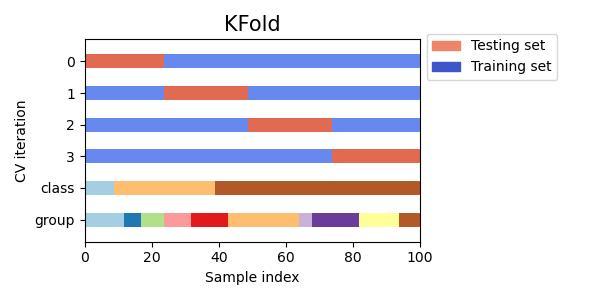
\includegraphics[width=.7\textwidth]{../figures/cv_kfold.png}
  \caption{A visualization of the splits of the data performed in cross validation. Here we see 4 $k$-folds which gives a total of 4 splits and iterations. \\
  \url{https://scikit-learn.org/stable/modules/cross_validation.html}}
  \label{fig:k_fold}
\end{figure}

\subsection{Study of $\lambda$ dependence for ridge and lasso regression}
To get the best possible predictions of our datasets we also implement lasso and ridge regression. These two methods are unlike OLS, dependent on a regularization parameter $\lambda$ where we have to compute which value that optimizes these two models. Similar to OLS we perform cross validation to find which degree of design matrix reduces the mean squared error of our predictions, only that we for ridge and lasso find the best $\lambda$ at the same time. This is because we for one degree would have one optimal $\lambda$ and for another degree have another. We therefore compute one cross validation for different values of $\lambda$ parameters for each degree. The degree and $\lambda$ giving the smallest MSE is then used for futher predictions

\subsection{Study of topography data}


\section{Results}
\section{Discussion}
\section{Conclusion}

\section{}

\end{document}
